\documentclass[pdflatex,sn-mathphys-num]{sn-jnl}

\usepackage{graphicx}
\usepackage{multirow}
\usepackage{amsmath,amssymb,amsfonts}
\usepackage{booktabs}
\usepackage{float}
\usepackage{algorithm}
\usepackage{algorithmicx}
\usepackage{algpseudocode}
\usepackage{tikz}
\usetikzlibrary{arrows.meta,positioning,fit,backgrounds}
\usepackage{needspace}

\raggedbottom
% Generated by make_numbers.py -- do not edit by hand.
\newcommand{\AblBaseline}{-0.0277}
\newcommand{\AblBestCell}{uniform / derived / all / tuned}
\newcommand{\AblBestRtwo}{0.7807}
\newcommand{\AblFull}{0.7622}
\newcommand{\AblNcells}{32}
\newcommand{\AblNorders}{24}
\newcommand{\CfgManualFull}{0.6925}
\newcommand{\CfgManualSub}{0.6901}
\newcommand{\CfgManualTopFull}{0.7438}
\newcommand{\CfgManualTopSub}{0.7155}
\newcommand{\CfgUniformFull}{0.7453}
\newcommand{\CfgUniformSub}{0.7423}
\newcommand{\CfgUniformTopFull}{0.7664}
\newcommand{\CfgUnscaledFull}{-0.0277}
\newcommand{\CfgUnscaledSub}{-0.0538}
\newcommand{\CvCorrhi}{0.719}
\newcommand{\CvCorrlo}{0.667}
\newcommand{\CvMean}{0.6931}
\newcommand{\CvSd}{0.0368}
\newcommand{\CvVOnehi}{0.765}
\newcommand{\CvVOnelo}{0.621}
\newcommand{\DSAmesBase}{0.6819}
\newcommand{\DSAmesFull}{0.8358}
\newcommand{\DSAmesFullUni}{0.8381}
\newcommand{\DSAmesN}{1022}
\newcommand{\DSAmesP}{36}
\newcommand{\DSAmesScal}{-0.1558}
\newcommand{\DSAmesSelect}{+0.1606}
\newcommand{\DSAmesTune}{+0.1491}
\newcommand{\DSAmesUniScal}{+0.1211}
\newcommand{\DSAmesUniSelect}{+0.0068}
\newcommand{\DSAmesUniTune}{+0.0283}
\newcommand{\DSCaliforniaBase}{0.5013}
\newcommand{\DSCaliforniaFull}{0.7563}
\newcommand{\DSCaliforniaFullUni}{0.7768}
\newcommand{\DSCaliforniaN}{10000}
\newcommand{\DSCaliforniaP}{18}
\newcommand{\DSCaliforniaScal}{+0.1616}
\newcommand{\DSCaliforniaSelect}{+0.0186}
\newcommand{\DSCaliforniaTune}{+0.0749}
\newcommand{\DSCaliforniaUniScal}{+0.1869}
\newcommand{\DSCaliforniaUniSelect}{+0.0157}
\newcommand{\DSCaliforniaUniTune}{+0.0730}
\newcommand{\DSKcHouseBase}{0.3888}
\newcommand{\DSKcHouseFull}{0.8092}
\newcommand{\DSKcHouseFullUni}{0.7806}
\newcommand{\DSKcHouseN}{10000}
\newcommand{\DSKcHouseP}{20}
\newcommand{\DSKcHouseScal}{+0.0805}
\newcommand{\DSKcHouseSelect}{+0.1197}
\newcommand{\DSKcHouseTune}{+0.2202}
\newcommand{\DSKcHouseUniScal}{+0.2710}
\newcommand{\DSKcHouseUniSelect}{+0.0053}
\newcommand{\DSKcHouseUniTune}{+0.1155}
\newcommand{\FlipA}{SVR uniform / raw8 / default / n=3000}
\newcommand{\FlipB}{SVR manual / top12 / tuned / full}
\newcommand{\FlipDiff}{-0.0271}
\newcommand{\FlipP}{0.166}
\newcommand{\FlipPuncorr}{0.007}
\newcommand{\GbmFull}{0.8384}
\newcommand{\GbmSmall}{0.8055}
\newcommand{\GridFits}{192}
\newcommand{\GridRtwo}{0.7806}
\newcommand{\GridSecs}{422}
\newcommand{\GridSecsMin}{7.0}
\newcommand{\KbelowPlateau}{0.5745}
\newcommand{\KbestAt}{10}
\newcommand{\KbestK}{10}
\newcommand{\KernLinear}{0.6469}
\newcommand{\KernPolyThree}{0.6650}
\newcommand{\KernPolyTwo}{0.6613}
\newcommand{\KernRbf}{0.7702}
\newcommand{\KernSigmoid}{0.3207}
\newcommand{\KmaxAt}{18}
\newcommand{\KminAt}{4}
\newcommand{\KnnFull}{0.7599}
\newcommand{\KnnSmall}{0.7179}
\newcommand{\KplateauFrom}{10}
\newcommand{\KplateauRange}{0.0045}
\newcommand{\KrangeHi}{0.7683}
\newcommand{\KrangeLo}{0.5745}
\newcommand{\MaxDeriv}{+0.5428}
\newcommand{\MaxScal}{+0.7202}
\newcommand{\MaxSelect}{+0.5937}
\newcommand{\MaxTune}{+0.5312}
\newcommand{\MinDeriv}{-0.0881}
\newcommand{\MinScal}{-0.0239}
\newcommand{\MinSelect}{-0.0029}
\newcommand{\MinTune}{+0.0152}
\newcommand{\NDatasets}{3}
\newcommand{\NFlipped}{2}
\newcommand{\NModels}{10}
\newcommand{\NOrderHoldsAuto}{1}
\newcommand{\NOrderHoldsUni}{3}
\newcommand{\NPairs}{21}
\newcommand{\NestedRandom}{0.7532}
\newcommand{\NestedRandomMax}{0.767}
\newcommand{\NestedRandomMin}{0.744}
\newcommand{\NestedSpatial}{-0.5344}
\newcommand{\NestedSpatialMax}{0.660}
\newcommand{\NestedSpatialMin}{-4.091}
\newcommand{\NystroemM}{2000}
\newcommand{\NystroemRtwo}{0.7673}
\newcommand{\NystroemSecs}{18}
\newcommand{\PairManualDiff}{+0.0242}
\newcommand{\PairManualP}{4.6\times 10^{-6}}
\newcommand{\PairManualPuncorr}{3.4\times 10^{-9}}
\newcommand{\PairRfDiff}{-0.0446}
\newcommand{\PairRfP}{9.3\times 10^{-5}}
\newcommand{\PairRfPuncorr}{9.4\times 10^{-8}}
\newcommand{\PairXgbDiff}{-0.0728}
\newcommand{\PairXgbP}{1.9\times 10^{-7}}
\newcommand{\PairXgbPuncorr}{1.2\times 10^{-10}}
\newcommand{\PreethiReportedMSE}{1.12}
\newcommand{\PreethiReportedRtwo}{0.15}
\newcommand{\RandSixtyRtwo}{0.7834}
\newcommand{\RandSixtySecs}{203}
\newcommand{\RandTwentyRtwo}{0.7702}
\newcommand{\RandTwentySecs}{100}
\newcommand{\RandTwoHundredRtwo}{0.7796}
\newcommand{\RandTwoHundredSecs}{1377}
\newcommand{\RandomCVmean}{0.7496}
\newcommand{\RangeDeriv}{0.6309}
\newcommand{\RangeScal}{0.7441}
\newcommand{\RangeSelect}{0.5966}
\newcommand{\RangeTune}{0.5160}
\newcommand{\RepScaledDefault}{0.737}
\newcommand{\RepScaledTuned}{0.766}
\newcommand{\RepScaledTunedMSE}{0.309}
\newcommand{\RepSeeds}{5}
\newcommand{\RepUnscaledDefault}{-0.020}
\newcommand{\RepUnscaledDefaultMSE}{1.343}
\newcommand{\RepUnscaledTuned}{0.514}
\newcommand{\RepUnscaledTunedMSE}{0.640}
\newcommand{\RfFull}{0.8171}
\newcommand{\RfSmall}{0.7610}
\newcommand{\RidgeFull}{0.6504}
\newcommand{\RidgeSmall}{0.6497}
\newcommand{\SearchBest}{random 60}
\newcommand{\SearchBestRtwo}{0.7834}
\newcommand{\SearchBestSecs}{203}
\newcommand{\SelectionOptimism}{0.0000}
\newcommand{\ShapDeriv}{0.1505}
\newcommand{\ShapScal}{0.2723}
\newcommand{\ShapSelect}{0.1789}
\newcommand{\ShapTune}{0.1882}
\newcommand{\SizeFull}{0.7813}
\newcommand{\SizeFullN}{14448}
\newcommand{\SizeFullRmse}{0.5382}
\newcommand{\SizeFullSecs}{8.3}
\newcommand{\SizeSmall}{0.6775}
\newcommand{\SizeSmallN}{1000}
\newcommand{\SizeThreeK}{0.7418}
\newcommand{\SizeThreeKrmse}{0.5848}
\newcommand{\SpatialCVmean}{0.2316}
\newcommand{\SpatialCVsd}{0.7525}
\newcommand{\SpatialOptimism}{0.5180}
\newcommand{\StatRho}{0.429}
\newcommand{\StatSplits}{10}
\newcommand{\StatSvrCIhi}{0.783}
\newcommand{\StatSvrCIlo}{0.769}
\newcommand{\StatSvrMean}{0.7757}
\newcommand{\StatSvrNBhi}{0.792}
\newcommand{\StatSvrNBlo}{0.759}
\newcommand{\StatSvrSd}{0.0099}
\newcommand{\StatSvrVOnehi}{0.795}
\newcommand{\StatSvrVOnelo}{0.756}
\newcommand{\SvrRankFull}{4}
\newcommand{\SvrRankSmall}{4}
\newcommand{\SvrRbfFull}{0.7702}
\newcommand{\SvrRbfSmall}{0.7501}
\newcommand{\ThreshRange}{0.0004}
\newcommand{\WeightMax}{0.7674}
\newcommand{\WeightMin}{0.7128}
\newcommand{\WeightMinOverlap}{10}
\newcommand{\WeightN}{66}
\newcommand{\WeightRange}{0.0546}
\newcommand{\XgbFull}{0.8483}
\newcommand{\XgbSmall}{0.8057}


\begin{document}

\title[Reassessing SVR on California Housing]{A Controlled Reassessment of Support Vector Regression on the California Housing Benchmark with Feature Scaling, Feature Selection and Hyperparameter Tuning}

\author*[1]{\fnm{Emmanuel} \sur{Adutwum}}
\email{eadutwum@soka.edu}

\affil*[1]{%
  \orgname{Soka University of America},
  \orgaddress{\city{Aliso Viejo}, \state{California}, \country{United States}}%
}

\maketitle

\begin{abstract}
\noindent Support Vector Regression (SVR) was recently reported as the weakest of six regressors on the California Housing benchmark by Preethi et al. (2025), who obtained an $R^2$ of approximately \PreethiReportedRtwo{} for SVR with an RBF kernel while linear, ridge and polynomial-ridge models reached approximately $0.58$. This paper asks whether that outcome is a property of the algorithm or of the configuration in which it was run, and answers the question by reproduction rather than by assertion. The configuration described in the prior study --- eight raw features, an RBF kernel, a grid over $C$ and $\varepsilon$ only, and no scaling step --- is re-run here: it yields $R^2 = \RepUnscaledDefault$ with library defaults and $R^2 = \RepUnscaledTuned$ when $C$ and $\varepsilon$ are tuned, bracketing the published value, whereas adding standardisation to the identical pipeline yields $R^2 = \RepScaledTuned$. A four-factor ablation over scaling, derived features, feature selection and hyperparameter tuning is then evaluated in every one of its \AblNcells{} cells, and each component is attributed an order-independent Shapley value; the apparent contribution of scaling varies by \RangeScal{} in $R^2$ across orderings, which is why single-path ablations should not be read as independent contributions. All ten comparison models are retrained with identical features, identical training rows and an identical tuning budget; differences are tested on \StatSplits{} common splits using the Nadeau--Bengio corrected resampled $t$-test, and the confidence interval formula used in the earlier version of this work is corrected. Spatially blocked cross-validation and feature selection performed inside every fold quantify how optimistic the random-split estimate is. The workflow is then applied unchanged to King County and Ames housing data. Two negative results are reported: the hand-assigned feature-specific scaling strategy does not outperform plain standardisation, and the tuned SVR remains behind gradient-boosted trees even at equal training size. Conclusions are restricted to the datasets and configurations examined here.
\end{abstract}

\keywords{Support Vector Regression, Feature Scaling, Ablation Analysis, Reproducibility, Spatial Cross-Validation, California Housing}

%============================================================================
\section{Introduction}\label{sec:intro}

\subsection{Background}
Estimating residential property value sits at the boundary of economics, urban planning and statistical learning. For several decades the dominant approach was the hedonic pricing model, which decomposes the value of a property into the implicit prices of its attributes \cite{rosen1974}. Hedonic regression offers an interpretable and theoretically grounded structure, but its linearity assumption becomes restrictive as datasets grow and the relationships between attributes and prices become less additive. Machine learning offers an alternative in which flexible function approximators are fitted without explicit distributional assumptions \cite{limsombunchai2004,fan2006,park2015}.

The California Housing dataset, derived from the 1990 United States Census and introduced to the statistical literature by Pace and Barry \cite{pace1997}, has become one of the most widely used regression benchmarks. It contains 20{,}640 census block groups described by eight numerical features, with the median house value of the block group as the target. It is distributed with scikit-learn \cite{pedregosa2011}, which makes any experiment on it straightforward to reproduce --- and therefore straightforward to check.

\subsection{The result under examination}\label{sec:the-result}
Preethi et al.\ \cite{preethi2025} compared six regression models on this dataset: linear regression, ridge regression, best polynomial ridge regression, lasso regression, elastic net regression, and SVR with an RBF kernel. They report that SVR performs worst, with the highest mean squared error and the lowest $R^2$, and that the linear, ridge and polynomial-ridge models each explain approximately 60\% of the variance.

Two features of that report matter here. First, the figure of approximately $0.60$ is the score of the \emph{linear family}, not of SVR: reading their Figs.~7 and 8, the SVR-RBF model attains $R^2 \approx \PreethiReportedRtwo$ with a mean squared error of approximately \PreethiReportedMSE{}, against $R^2 \approx 0.58$ and MSE $\approx 0.55$ for the leading models. An earlier version of the present work quoted $0.60$ as the SVR result; that reading was incorrect and is corrected here. Second, their methodology section describes loading the data, splitting it, fitting the six models, tuning SVR's $C$ and $\varepsilon$ with a grid search, and evaluating with $k$-fold cross-validation. No feature scaling step is described anywhere in the paper. Since the RBF kernel acts on Euclidean distances between feature vectors, a pipeline in which \texttt{Population} ranges over $[3,\,35{,}682]$ while \texttt{AveBedrms} ranges over $[0.33,\,34]$ places almost all of the kernel's sensitivity on a single feature.

\subsection{Research questions}\label{sec:questions}
This study is a controlled reassessment of that specific result, not a general claim about SVR. It asks four questions:

\begin{enumerate}
\item[Q1] Can the reported SVR result be reproduced from the configuration described, and what does the identical pipeline yield when a scaling step is added? (Section~\ref{sec:res-reproduction})
\item[Q2] When every model is given the same features, the same training rows and the same tuning budget, where does a tuned SVR actually rank, and are the differences statistically distinguishable? (Sections~\ref{sec:res-models} and \ref{sec:res-stats})
\item[Q3] How much of the improvement is attributable to each pipeline component once the attribution is made independent of the order in which components are applied? (Section~\ref{sec:res-ablation})
\item[Q4] How much of the measured performance survives spatially blocked validation and feature selection performed inside the resampling loop, and does the pattern hold on other datasets? (Sections~\ref{sec:res-validation} and \ref{sec:res-datasets})
\end{enumerate}

\subsection{Contributions}\label{sec:contributions}
The contribution of this paper is methodological and diagnostic rather than algorithmic. No new learning algorithm is proposed. Specifically:

\begin{enumerate}
\item A corrected reading of the prior result, and a direct reproduction of the configuration described there, run over several seeds and reported against the published values (Section~\ref{sec:res-reproduction}).
\item An explicit statement of the preprocessing workflow as a staged procedure with defined inputs and outputs (Section~\ref{sec:workflow}), including a distribution-aware rule that assigns a scaler to each feature from training-fold statistics alone (Algorithm~\ref{alg:scaler}). In the earlier version this assignment was a hand-made table specific to one dataset; as a rule it can be stated, audited and applied elsewhere.
\item An order-independent ablation procedure for preprocessing pipelines: the full factorial design is evaluated and each component receives a Shapley value, which removes the dependence of the reported increments on the sequence in which components are introduced (Section~\ref{sec:ablation-protocol}).
\item An evaluation protocol with a corrected confidence interval, paired tests on identical splits using the Nadeau--Bengio correction \cite{nadeau2003}, spatially blocked cross-validation \cite{roberts2017}, and feature selection repeated inside every fold \cite{varma2006,ambroise2002}.
\item Two negative results, reported because they qualify the earlier version's claims: the feature-specific scaling strategy does not outperform uniform standardisation on this dataset, and the derived features contribute little once selection and tuning are in place.
\end{enumerate}

\subsection{Scope of the claims}\label{sec:scope}
All quantitative claims in this paper are restricted to the datasets, feature sets, search spaces and implementations described in Section~\ref{sec:setup}. That feature scaling is necessary for distance-based kernels is a long-established result \cite{sola1997,hsu2003,singh2020}; this paper does not claim it as a discovery. What is offered is a controlled measurement of how much of one specific published comparison is attributable to that omission, and a protocol under which such a measurement can be repeated.

%============================================================================
\section{Related work}\label{sec:related}

\subsection{Feature scaling in kernel methods}\label{sec:rw-scaling}
The sensitivity of kernel methods to input scaling is documented from the earliest practical guides onward. Hsu et al.\ \cite{hsu2003} make normalisation the first step of their recommended SVM procedure; Smola and Sch\"olkopf \cite{smola2004} note that the kernel is a function of distances in input space and therefore inherits any anisotropy in the feature scales. Sola and Sevilla \cite{sola1997} demonstrated the effect for neural networks on industrial data, and Singh and Singh \cite{singh2020} survey normalisation techniques and quantify their effect across classifiers. Fern\'andez-Delgado et al.\ \cite{fernandez2014} report, over 121 datasets, that kernel machines are considerably more sensitive to preprocessing quality than tree ensembles, which are invariant to monotone transformations of individual features. The present study is positioned within this literature as a reassessment of one published comparison, not as a new finding about scaling.

\subsection{The California Housing benchmark}\label{sec:rw-benchmark}
Pace and Barry \cite{pace1997} introduced the data in a spatial-autoregression study and reported that spatial dependence carries substantial predictive information. Subsequent comparative studies routinely place gradient-boosted trees at the top of the ranking on this benchmark \cite{chen2016}. Preethi et al.\ \cite{preethi2025} are the immediate point of comparison for this work; their study is discussed in Section~\ref{sec:the-result} and reproduced in Section~\ref{sec:res-reproduction}. Because the dataset is a geographic sample, the validation design matters: neighbouring block groups are strongly dependent, so a random partition places near-duplicates on both sides of the split. Roberts et al.\ \cite{roberts2017} and Meyer et al.\ \cite{meyer2018} show that random cross-validation is optimistic for spatially structured data and recommend blocked designs, which are adopted in Section~\ref{sec:res-validation}.

\subsection{Comparing models and attributing gains}\label{sec:rw-compare}
Comparing learners on a single test split conflates a genuine difference with partition noise. Dietterich \cite{dietterich1998} analyses the error rates of common comparison procedures, and Nadeau and Bengio \cite{nadeau2003} show that the ordinary paired $t$-test applied to repeated random splits is anti-conservative because the resampled training sets overlap; they derive the variance correction used in Section~\ref{sec:res-stats}. Dem\v{s}ar \cite{demsar2006} extends the discussion to comparisons over many datasets. On the selection side, Ambroise and McLachlan \cite{ambroise2002} and Varma and Simon \cite{varma2006} show that performing feature selection or model selection outside the resampling loop produces optimistically biased estimates, and Cawley and Talbot \cite{cawley2010} document the same effect for hyperparameter selection. Attribution of a pipeline's gain to its components is a cooperative-game problem: the Shapley value \cite{shapley1953} is the unique attribution that is order-independent and adds up to the total, and it is used here for exactly that reason.

%============================================================================
\section{Proposed workflow}\label{sec:workflow}

This section defines the workflow before any data are analysed, as an explicit sequence of stages with stated inputs and outputs. Figure~\ref{fig:pipeline} shows the stages and the data that flows between them, and Table~\ref{tab:workflow} states the same information in tabular form. The essential property of the design is that every stage that estimates anything from data --- feature ranking, scaler assignment, scaler parameters, hyperparameters --- is fitted on the training portion only, and is re-fitted from scratch inside every fold of every resampling scheme used in Section~\ref{sec:results}.

\begin{figure}[htbp]
\centering
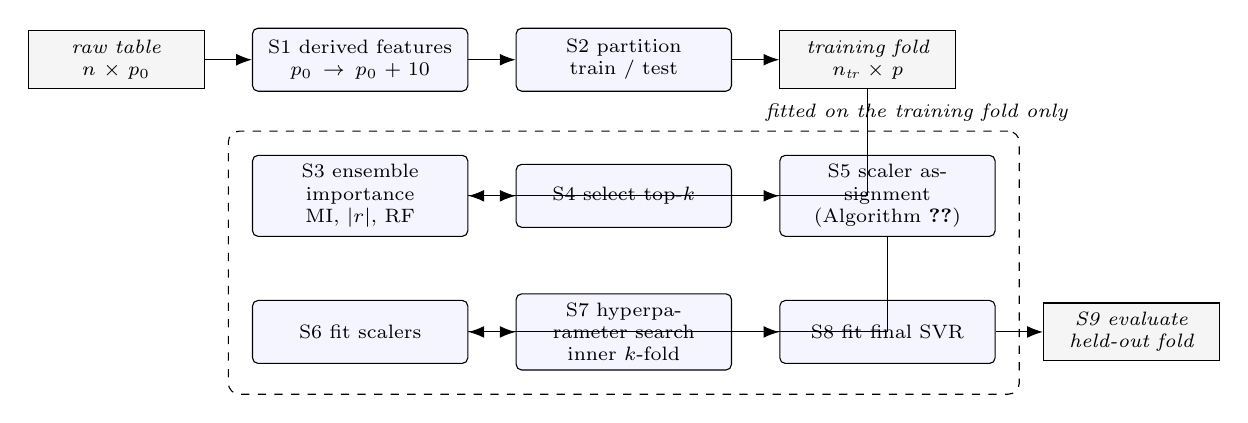
\begin{tikzpicture}[
  node distance=4mm and 6mm,
  box/.style={draw, rounded corners=2pt, align=center, font=\scriptsize,
              minimum height=8mm, text width=25mm, fill=blue!4},
  data/.style={draw, align=center, font=\scriptsize\itshape, text width=20mm,
               minimum height=7mm, fill=black!4},
  arr/.style={-{Latex[length=2mm]}, thin}]

\node[data] (raw) {raw table\\$n \times p_0$};
\node[box, right=of raw] (derive) {S1 derived features\\$p_0 \to p_0 + 10$};
\node[box, right=of derive] (split) {S2 partition\\train / test};
\node[data, right=of split] (tr) {training fold\\$n_{\text{tr}} \times p$};

\node[box, below=8mm of derive] (rank) {S3 ensemble importance\\MI, $|r|$, RF};
\node[box, right=of rank] (select) {S4 select top-$k$};
\node[box, right=of select] (assign) {S5 scaler assignment\\(Algorithm~\ref{alg:scaler})};
\node[box, below=8mm of rank] (fit) {S6 fit scalers};
\node[box, right=of fit] (search) {S7 hyperparameter search\\inner $k$-fold};
\node[box, right=of search] (final) {S8 fit final SVR};
\node[data, right=of final] (eval) {S9 evaluate\\held-out fold};

\draw[arr] (raw) -- (derive);
\draw[arr] (derive) -- (split);
\draw[arr] (split) -- (tr);
\draw[arr] (tr.south) |- (rank.east);
\draw[arr] (rank) -- (select);
\draw[arr] (select) -- (assign);
\draw[arr] (assign.south) |- (fit.east);
\draw[arr] (fit) -- (search);
\draw[arr] (search) -- (final);
\draw[arr] (final) -- (eval);

\begin{scope}[on background layer]
\node[draw, dashed, rounded corners, fit=(rank)(select)(assign)(fit)(search)(final),
      inner sep=3mm, label={[font=\scriptsize\itshape]above right:fitted on the training fold only}] {};
\end{scope}
\end{tikzpicture}
\caption{The workflow evaluated in this paper. Stages S3--S8 are fitted using the training fold alone and are re-fitted inside every fold of every resampling scheme, so no quantity estimated from held-out data enters the model. Stage S1 is a row-wise transformation and carries no fitted state.}
\label{fig:pipeline}
\end{figure}

\begin{table}[htbp]
\centering
\caption{The workflow of Fig.~\ref{fig:pipeline} stated as stages with explicit inputs and outputs. ``Fitted state'' is the information a stage estimates from data; every such stage is re-fitted on the training portion of each fold.}\label{tab:workflow}
\small
\begin{tabular}{llll}
\toprule
Stage & Input & Output & Fitted state \\
\midrule
S1 derived features & raw table $n \times p_0$ & table $n \times (p_0{+}10)$ & none (row-wise) \\
S2 partition & full table & train / test folds & fold indices \\
S3 ensemble importance & training fold & score $s_j$ per feature & MI, $|r|$, RF model \\
S4 selection & scores $s_j$ & index set of size $k$ & selected indices \\
S5 scaler assignment & training fold & scaler type per feature & $\mathrm{out}_j$, $g_j$ \\
S6 scaler fitting & training fold, assignment & scaled training matrix & scaler parameters \\
S7 hyperparameter search & scaled training fold & $(C, \varepsilon, \gamma)$ & inner CV scores \\
S8 final fit & scaled training fold, $(C,\varepsilon,\gamma)$ & fitted SVR & support vectors, $\alpha$, $b$ \\
S9 evaluation & held-out fold, fitted pipeline & $R^2$, RMSE, MAE & none \\
\bottomrule
\end{tabular}
\end{table}


\subsection{Support Vector Regression}\label{sec:svr}
SVR \cite{drucker1997,smola2004,vapnik1995} fits a function of the form
\begin{equation}
f(\mathbf{x}) = \mathbf{w}^{\top}\phi(\mathbf{x}) + b ,
\label{eq:svr-primal-fn}
\end{equation}
where $\mathbf{x} \in \mathbb{R}^{p}$ is a feature vector, $\phi : \mathbb{R}^{p} \to \mathcal{H}$ maps it into a reproducing kernel Hilbert space, $\mathbf{w} \in \mathcal{H}$ is the weight vector in that space and $b \in \mathbb{R}$ is an intercept. Given training pairs $\{(\mathbf{x}_i, y_i)\}_{i=1}^{n}$ with $y_i \in \mathbb{R}$, the parameters solve
\begin{equation}
\min_{\mathbf{w},\,b,\,\xi,\,\xi^{*}} \;
\frac{1}{2}\lVert \mathbf{w} \rVert^{2}
+ C \sum_{i=1}^{n} \left( \xi_i + \xi_i^{*} \right)
\label{eq:svr-objective}
\end{equation}
subject to
\begin{align}
y_i - \mathbf{w}^{\top}\phi(\mathbf{x}_i) - b &\le \varepsilon + \xi_i, \label{eq:svr-c1}\\
\mathbf{w}^{\top}\phi(\mathbf{x}_i) + b - y_i &\le \varepsilon + \xi_i^{*}, \label{eq:svr-c2}\\
\xi_i,\; \xi_i^{*} &\ge 0, \qquad i = 1,\dots,n. \label{eq:svr-c3}
\end{align}
Here $\lVert \mathbf{w} \rVert^{2}$ is the squared norm of $\mathbf{w}$ and controls the flatness of $f$; $\varepsilon \ge 0$ is the half-width of the insensitive tube inside which residuals incur no loss; $\xi_i$ and $\xi_i^{*}$ are slack variables measuring how far the $i$-th residual falls above and below the tube; and $C > 0$ weights the total slack against flatness. Solving the dual of \eqref{eq:svr-objective} gives
\begin{equation}
f(\mathbf{x}) = \sum_{i=1}^{n} \left( \alpha_i - \alpha_i^{*} \right) K(\mathbf{x}_i, \mathbf{x}) + b ,
\label{eq:svr-dual}
\end{equation}
where $\alpha_i, \alpha_i^{*} \in [0, C]$ are the dual coefficients and $K(\cdot,\cdot)$ is the kernel. Points with $\alpha_i - \alpha_i^{*} \neq 0$ are the support vectors. The kernels evaluated in Section~\ref{sec:res-kernels} are
\begin{align}
K_{\text{rbf}}(\mathbf{x}, \mathbf{x}') &= \exp\!\left( -\gamma \lVert \mathbf{x} - \mathbf{x}' \rVert^{2} \right), \label{eq:k-rbf}\\
K_{\text{lin}}(\mathbf{x}, \mathbf{x}') &= \mathbf{x}^{\top}\mathbf{x}', \label{eq:k-lin}\\
K_{\text{poly}}(\mathbf{x}, \mathbf{x}') &= \left( \gamma\, \mathbf{x}^{\top}\mathbf{x}' + r \right)^{d}, \label{eq:k-poly}
\end{align}
with kernel width $\gamma > 0$, offset $r$ and degree $d$. Equation~\eqref{eq:k-rbf} makes the dependence on scaling explicit: the kernel is a function of the squared Euclidean distance, so a feature whose numerical range is three orders of magnitude larger than the others dominates $\lVert \mathbf{x} - \mathbf{x}' \rVert^{2}$ and the remaining features have almost no influence on the fitted function. All symbols used above are collected in Table~\ref{tab:notation}.

\begin{table}[htbp]
\centering
\caption{Notation used in Section~\ref{sec:svr}.}\label{tab:notation}
\small
\begin{tabular}{ll}
\toprule
Symbol & Meaning \\
\midrule
$n$, $p$ & number of training observations; number of features \\
$\mathbf{x}_i \in \mathbb{R}^{p}$, $y_i \in \mathbb{R}$ & $i$-th feature vector and its target value \\
$\phi(\cdot)$ & map from input space into the kernel feature space $\mathcal{H}$ \\
$\mathbf{w}$, $b$ & weight vector in $\mathcal{H}$ and intercept of Eq.~\eqref{eq:svr-primal-fn} \\
$\lVert \mathbf{w} \rVert^{2}$ & squared norm of $\mathbf{w}$; smaller values give a flatter function \\
$\varepsilon$ & half-width of the insensitive tube; residuals inside it incur no loss \\
$\xi_i,\ \xi_i^{*}$ & slack variables for violations above and below the tube \\
$C$ & regularisation constant weighting total slack against flatness \\
$\alpha_i,\ \alpha_i^{*} \in [0, C]$ & dual coefficients; non-zero values identify support vectors \\
$K(\cdot,\cdot)$ & kernel function \\
$\gamma$ & kernel width of the RBF and polynomial kernels \\
$d$, $r$ & degree and offset of the polynomial kernel \\
$s_j$ & pooled ensemble importance of feature $j$, Eq.~\eqref{eq:ensemble} \\
$k$ & number of features retained by Stage S4 \\
$\mathrm{out}_j$, $g_j$ & outlier fraction and skewness of feature $j$ used by Algorithm~\ref{alg:scaler} \\
$\varphi_c$ & Shapley value of pipeline component $c$, Eq.~\eqref{eq:shapley} \\
$J$ & number of resampled splits in the repeated-split analysis \\
\bottomrule
\end{tabular}
\end{table}


\subsection{Stage S1: derived features}\label{sec:derived}
Ten features are constructed from the eight raw inputs by row-wise arithmetic; the transformation has no fitted parameters, so it is applied before partitioning without any leakage. Table~\ref{tab:derived} gives each definition together with the reasoning behind it. Two of them require comment, because their geographic interpretation was questioned in review. \emph{Coastal proximity} is defined as $|\text{Latitude} - 34.05|$, the absolute latitude difference from a reference latitude near the Los Angeles coastline. This is a one-dimensional proxy: it measures north--south displacement from a southern reference point and does not measure distance to the coast, which would require the coastline geometry and both coordinates. \emph{Location score}, defined as $(\text{Latitude} \times \text{Longitude})/1000$, is an interaction term between the two coordinates rather than a geographic quantity with units; it is retained because the ensemble ranking assigns it non-trivial importance, but it should be read as an unnamed coordinate interaction, not as a location measure. Both are candidate features whose value is decided empirically by Stage S4, and Section~\ref{sec:res-ablation} reports how much the derived block contributes once selection and tuning are present.

\begin{table}[htbp]
\centering
\caption{The ten derived features constructed in Stage S1, with their definitions. All are row-wise functions of the eight raw inputs and introduce no fitted state. The unit-offset denominators avoid division by values near zero.}\label{tab:derived}
\small
\begin{tabular}{lll}
\toprule
Feature & Definition & Intended reading \\
\midrule
Income\_per\_Room & $\text{MedInc} / (\text{AveRooms} + 1)$ & purchasing power per unit of dwelling size \\
Room\_Value\_Score & $\text{MedInc} \times \text{AveRooms}$ & interaction of income and dwelling size \\
Location\_Score & $(\text{Latitude} \times \text{Longitude})/1000$ & coordinate interaction (no geographic unit) \\
Coastal\_Proximity & $|\text{Latitude} - 34.05|$ & north--south displacement from a southern reference \\
Bedroom\_Ratio & $\text{AveBedrms} / (\text{AveRooms} + 1)$ & proxy for dwelling type \\
Population\_Density & $\text{Population} / (\text{AveOccup} + 1)$ & block-group density approximation \\
Age\_Income\_Interaction & $\text{HouseAge} \times \text{MedInc}$ & separates older affluent from older low-income stock \\
Modernization\_Score & $\text{MedInc} / (\text{HouseAge} + 1)$ & income relative to housing-stock age \\
Rooms\_per\_Person & $\text{AveRooms} / (\text{AveOccup} + 1)$ & space per occupant \\
Income\_Density & $(\text{MedInc} \times \text{Population})/1000$ & aggregate purchasing power of the block group \\
\bottomrule
\end{tabular}
\end{table}


\subsection{Stages S3--S4: ensemble importance and selection}\label{sec:selection}
Three scores are computed on the training fold: mutual information $\mathrm{MI}(X_j; Y)$ estimated by the $k$-nearest-neighbour method, the absolute Pearson correlation $|r(X_j, Y)|$, and the impurity-based importance of a random forest \cite{breiman2001} with 100 trees. Each score vector is min--max normalised to $[0,1]$ and the three are pooled,
\begin{equation}
s_j = w_{\text{mi}} \, \widetilde{\mathrm{MI}}_j + w_{r} \, \widetilde{|r|}_j + w_{\text{rf}} \, \widetilde{\mathrm{RF}}_j ,
\qquad w_{\text{mi}} + w_{r} + w_{\text{rf}} = 1 ,
\label{eq:ensemble}
\end{equation}
and the $k$ features with the largest $s_j$ are retained. The defaults are $(w_{\text{mi}}, w_{r}, w_{\text{rf}}) = (0.4, 0.3, 0.3)$ and $k = 12$. These constants were chosen by hand and have no theoretical justification; Section~\ref{sec:res-sensitivity} therefore sweeps the entire weight simplex and a range of $k$ and reports how much the result depends on them. Where a general rule is needed --- for instance when the workflow is applied to a dataset with a different number of columns in Section~\ref{sec:res-datasets} --- $k$ is set to $\lceil 2p/3 \rceil$, which reproduces $k = 12$ for the eighteen columns of the augmented California table.

\subsection{Stage S5: distribution-aware scaler assignment}\label{sec:scaler}
The earlier version of this work assigned one of three scalers to each feature using a hand-written table. That table cannot be applied to another dataset and cannot be checked, so the assignment is restated here as a rule evaluated on training-fold statistics. For each feature the rule computes the fraction of observations beyond $1.5$ interquartile ranges from the quartiles, $\mathrm{out}_j$, and the sample skewness $g_j$, and assigns a scaler accordingly (Algorithm~\ref{alg:scaler}). The thresholds $\tau_{\text{out}} = 0.05$, $\tau_{\text{skew}} = 2$ and $\tau_{\text{bnd}} = 0.5$ are fixed in advance and swept in Section~\ref{sec:res-sensitivity}.

\begin{algorithm}[htbp]
\caption{Distribution-aware scaler assignment (Stage S5), fitted on the training fold}
\label{alg:scaler}
\begin{algorithmic}[1]
\Require training matrix $X^{\text{tr}} \in \mathbb{R}^{n_{\text{tr}} \times p}$; thresholds $\tau_{\text{out}}, \tau_{\text{skew}}, \tau_{\text{bnd}}$
\Ensure a fitted scaler $T_j$ for each feature $j$
\For{$j = 1$ to $p$}
  \State $q_1, q_3 \gets$ first and third quartiles of column $j$; \; $\mathrm{IQR} \gets q_3 - q_1$
  \State $\mathrm{out}_j \gets$ fraction of entries outside $[\,q_1 - 1.5\,\mathrm{IQR},\; q_3 + 1.5\,\mathrm{IQR}\,]$
  \State $g_j \gets$ sample skewness of column $j$
  \If{$\mathrm{out}_j > \tau_{\text{out}}$ \textbf{or} $|g_j| > \tau_{\text{skew}}$}
    \State $T_j \gets$ \textsc{RobustScaler} \Comment{heavy tails; centre and scale by median and IQR}
  \ElsIf{$\mathrm{out}_j = 0$ \textbf{and} $|g_j| < \tau_{\text{bnd}}$}
    \State $T_j \gets$ \textsc{MinMaxScaler} \Comment{bounded and near-symmetric}
  \Else
    \State $T_j \gets$ \textsc{StandardScaler}
  \EndIf
  \State fit $T_j$ on column $j$ of $X^{\text{tr}}$
\EndFor
\end{algorithmic}
\end{algorithm}

\subsection{Stages S7--S8: hyperparameter search}\label{sec:tuning}
Hyperparameters are selected by cross-validated search on the training fold only. Two search strategies are used and compared in Section~\ref{sec:res-kernels}: an exhaustive grid over the discretised space $C \in \{0.1, 1, 10, 100\}$, $\varepsilon \in \{0.01, 0.1, 0.5, 1.0\}$, $\gamma \in \{\text{scale}, \text{auto}, 0.1, 1\}$, and a randomised search \cite{bergstra2012} that draws $C \sim \mathrm{LogUniform}(0.1, 300)$, $\varepsilon \sim \mathrm{LogUniform}(0.01, 1)$ and $\gamma \sim \mathrm{LogUniform}(10^{-3}, 1)$. The earlier version drew from a discretised space inside a randomised search, which wastes the main advantage of randomised search; the two strategies are therefore reported side by side, with fit counts and wall-clock times, so the choice can be made on evidence.

\subsection{Evaluation protocol}\label{sec:eval-protocol}
Four estimates of generalisation are reported, and they are not interchangeable:

\begin{enumerate}
\item \textbf{Single held-out split.} A stratified 70/30 partition, stratified on target deciles so that the two halves have comparable target distributions. Stratification is not required in regression; it is used here only to remove one source of variation between configurations that are being compared, and the repeated-split analysis below does not depend on it.
\item \textbf{Repeated splits.} The entire workflow --- including feature ranking, selection, scaler assignment and hyperparameter search --- is re-run on \StatSplits{} independent partitions. Reported as a mean with a confidence interval for that mean.
\item \textbf{Random and spatially blocked cross-validation.} $k$-means on the standardised block-group centroids partitions California into ten contiguous regions, which are then used as folds, so that every evaluation is made on a region the model has not seen \cite{roberts2017}.
\item \textbf{Nested cross-validation.} Hyperparameter search and feature selection are performed inside each outer fold, giving an estimate that is not contaminated by selection \cite{varma2006,cawley2010}.
\end{enumerate}

\paragraph{Interval estimation.} For $J$ resampled estimates $\hat{r}_1, \dots, \hat{r}_J$ with mean $\bar{r}$ and sample standard deviation $s$, the earlier version reported $\bar{r} \pm 1.96\,s$. That expression is a prediction interval for a single fold, not a confidence interval for the mean, and it overstates the width by a factor of approximately $\sqrt{J}$. The correct interval for the mean is
\begin{equation}
\bar{r} \pm t_{0.975,\,J-1} \, \frac{s}{\sqrt{J}} .
\label{eq:ci-correct}
\end{equation}
Equation~\eqref{eq:ci-correct} still assumes independent estimates, which resampled splits are not: they share training data. Following Nadeau and Bengio \cite{nadeau2003}, the corrected variance for $J$ random splits with $n_{\text{te}}$ test and $n_{\text{tr}}$ training observations replaces $s^2/J$ by
\begin{equation}
\hat{\sigma}^{2}_{\text{corr}} = s^{2}\left( \frac{1}{J} + \frac{n_{\text{te}}}{n_{\text{tr}}} \right),
\label{eq:nb-var}
\end{equation}
which for the present design ($n_{\text{te}}/n_{\text{tr}} = \StatRho$) inflates the standard error substantially. Both \eqref{eq:ci-correct} and \eqref{eq:nb-var} are reported in Section~\ref{sec:res-stats}, alongside the incorrect v1 expression, so the size of the original error is visible.

\paragraph{Paired comparison.} Models are compared on identical splits. For each split the difference $d_i = r_i^{(A)} - r_i^{(B)}$ is formed, and the corrected statistic
\begin{equation}
t = \frac{\bar{d}}{s_d \sqrt{\dfrac{1}{J} + \dfrac{n_{\text{te}}}{n_{\text{tr}}}}}
\label{eq:nb-t}
\end{equation}
is referred to a $t$ distribution with $J-1$ degrees of freedom \cite{nadeau2003}. The uncorrected paired $t$-test and the Wilcoxon signed-rank test are reported alongside it for reference \cite{dietterich1998}.

\subsection{Ablation protocol}\label{sec:ablation-protocol}
The earlier version applied components in one order --- scaling, then feature engineering, then tuning --- and reported the increment at each step as that component's contribution. Two problems follow. First, increments measured along a single path depend on the path: a component applied first absorbs all of the interaction it shares with later components. Second, ``feature engineering'' bundled two distinct operations, constructing derived features and selecting a subset.

The design used here separates four binary components: scaling $S$, derived features $D$, selection $K$ and tuning $T$. All $2^4$ combinations are evaluated (with $S$ taking each of four levels, giving \AblNcells{} fitted configurations), every one of the $4! = \AblNorders$ orderings is traced, and each component $c$ receives the Shapley value \cite{shapley1953}
\begin{equation}
\varphi_c = \sum_{\mathcal{S} \subseteq \mathcal{C} \setminus \{c\}}
\frac{|\mathcal{S}|!\,\bigl(|\mathcal{C}| - |\mathcal{S}| - 1\bigr)!}{|\mathcal{C}|!}
\Bigl[ v\bigl(\mathcal{S} \cup \{c\}\bigr) - v(\mathcal{S}) \Bigr],
\label{eq:shapley}
\end{equation}
where $\mathcal{C}$ is the set of components and $v(\mathcal{S})$ is the test $R^2$ of the configuration in which exactly the components in $\mathcal{S}$ are enabled. The values $\varphi_c$ are order-independent and satisfy $\sum_c \varphi_c = v(\mathcal{C}) - v(\emptyset)$, so they can be read as contributions in a way that single-path increments cannot.

%============================================================================
\section{Experimental setup}\label{sec:setup}

\subsection{Datasets}\label{sec:datasets}
Three tabular regression datasets are used. \textbf{California Housing} \cite{pace1997,pedregosa2011} contains 20{,}640 census block groups with eight numerical features and, as the target, the median house value of the block group in units of \$100{,}000. It has no missing values and no duplicate rows. Its target is capped at \$500{,}001 by the census recording procedure, which produces a spike of 965 block groups at the upper limit; this artefact is present in the prior study as well and therefore does not confound the comparison, but it does bound the achievable fit. \textbf{King County house sales} contains 21{,}613 individual transactions with 18 numerical predictors, including coordinates, and the sale price as target. \textbf{Ames Housing} \cite{decock2011} contains 1{,}460 sales with 36 usable numerical predictors after columns that are more than 20\% missing are dropped and the remainder median-imputed. Both additional datasets are retrieved from OpenML; targets are expressed in units of \$100{,}000 so that error metrics are numerically comparable across datasets. Table~\ref{tab:datasets} reports the resulting sizes.

The characteristics of the California features are what motivate the scaling stage: \texttt{Population} spans $[3,\,35{,}682]$, \texttt{AveOccup} spans $[0.69,\,1{,}243]$ and \texttt{AveRooms} spans $[0.85,\,141.9]$, while \texttt{MedInc} spans $[0.50,\,15.0]$ and the two coordinates span less than ten units each. Under an unscaled RBF kernel the first three features determine essentially the whole distance computation.

\subsection{Implementation and reproducibility}
All experiments run under Python 3.11 with scikit-learn 1.8, XGBoost 1.7, NumPy 1.26 and SciPy, on an eight-core Apple silicon workstation without GPU acceleration. SVR is scikit-learn's \texttt{SVR}, backed by LIBSVM \cite{chang2011}. Random seeds are fixed and reported with every result: the single-split experiments use seed 42, and the repeated-split experiments use seeds $0$ to $\StatSplits{}-1$. Each experiment writes a JSON record of every configuration, metric, selected feature set, chosen hyperparameter and wall-clock time; the tables and figures of this paper are generated directly from those records, so the numbers in the text, the tables and the figures cannot diverge. Code and result records are available at the repository given under Data Availability.

\subsection{What is held fixed}\label{sec:fixed}
Within each comparison exactly one factor varies. In Section~\ref{sec:res-models} all ten models receive the same twelve features, the same training rows and the same search budget of 20 randomised iterations with three-fold cross-validation. In Section~\ref{sec:res-ablation} every cell is fitted on the full training set with the same grid. In Section~\ref{sec:res-datasets} the scaler rule, the selection rule and the search space are identical across datasets, with no dataset-specific adjustment; the only difference is the training-size cap, which is applied equally to every cell within a dataset.

%============================================================================
\section{Results}\label{sec:results}

\subsection{Reproducing the prior configuration}\label{sec:res-reproduction}
Table~\ref{tab:reproduction} reports the configuration described by Preethi et al.\ \cite{preethi2025}, re-run over \RepSeeds{} seeds with an 80/20 partition, the eight raw features and an RBF kernel. With library defaults and no scaling the model attains $R^2 = \RepUnscaledDefault$ (MSE $= \RepUnscaledDefaultMSE$); with $C$ and $\varepsilon$ grid-searched and $\gamma$ left at its default, it attains $R^2 = \RepUnscaledTuned$ (MSE $= \RepUnscaledTunedMSE$). The published value of $R^2 \approx \PreethiReportedRtwo$ falls between these two, which is what one expects from an unscaled pipeline with a limited search. Adding a single standardisation step to the same pipeline, changing nothing else, yields $R^2 = \RepScaledDefault$ with defaults and $R^2 = \RepScaledTuned$ when tuned.

This answers Q1 and also resolves an inconsistency in the earlier version of this work. That version compared an unscaled baseline of $R^2 = -0.054$ against a figure of $0.60$ attributed to the prior study's SVR, and the gap between them was never explained. It could not be: as Section~\ref{sec:the-result} sets out, $0.60$ was the score of the prior study's linear models, and its SVR result is approximately \PreethiReportedRtwo{}. Once the correct value is used, the unscaled configurations reproduced here bracket it, and no unexplained gap remains. Figure~\ref{fig:reproduction} shows the four configurations against the published value.

\begin{figure}[htbp]
\centering
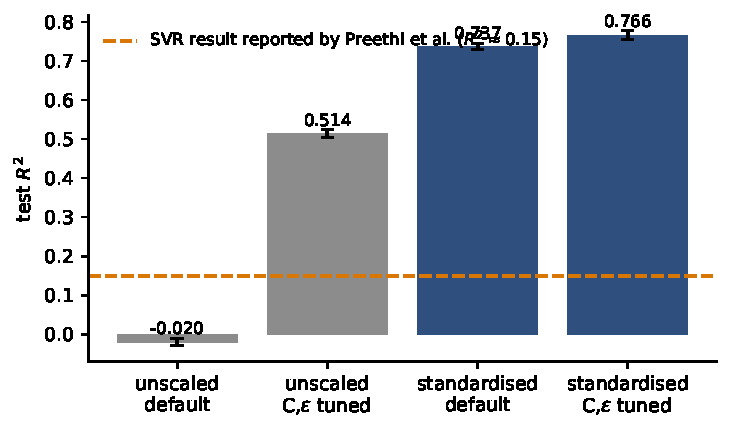
\includegraphics[width=0.78\textwidth]{figures/fig_reproduction.pdf}
\caption{Reproduction of the prior configuration. Bars are means over \RepSeeds{} seeds with standard-deviation whiskers; the dashed line is the SVR result reported by Preethi et al.\ \cite{preethi2025}, read from their Fig.~8. The two unscaled configurations bracket the published value; both standardised configurations are far above it.}
\label{fig:reproduction}
\end{figure}

\begin{table}[htbp]
\centering
\caption{Reproduction of the SVR configuration described by Preethi et al. (2025). Eight raw features, RBF kernel, 80/20 split, mean $\pm$ standard deviation over 5 seeds.}\label{tab:reproduction}
\small
\begin{tabular}{lccc}
\toprule
Configuration & Test $R^2$ & Test MSE & Gap to reported $R^2$ \\
\midrule
Unscaled, library defaults & $-0.020 \pm 0.010$ & $1.343$ & $-0.170$ \\
Unscaled, $C$ and $\varepsilon$ grid-searched & $0.514 \pm 0.010$ & $0.640$ & $+0.364$ \\
Standardised, library defaults & $0.737 \pm 0.008$ & $0.346$ & $+0.587$ \\
Standardised, $C$ and $\varepsilon$ grid-searched & $0.766 \pm 0.011$ & $0.309$ & $+0.616$ \\
\midrule Reported by Preethi et al. & $\approx 0.15$ & $\approx 1.12$ & --- \\
\bottomrule
\end{tabular}
\begin{flushleft}\footnotesize The values attributed to Preethi et al. are read from their Figs.~7 and 8; their paper reports no numerical table. Their stated procedure tunes $C$ and $\varepsilon$ only, leaving $\gamma$ at the library default, and describes no scaling step.\end{flushleft}
\end{table}

Table~\ref{tab:configurations} extends this to the full set of scaling, feature-set and training-size combinations on one identical split, which is the direct comparison the editor requested between the prior study's uniform scaling and the feature-specific strategy proposed in the earlier version of this work. Uniform standardisation of the eight raw features gives $R^2 = \CfgUniformFull$ on the full training set, while the hand-assigned feature-specific strategy gives $\CfgManualFull$ on the same split and the same features. The feature-specific strategy is therefore not an improvement over uniform standardisation on this dataset; it is worse by approximately $0.05$ in $R^2$. This is the first of the two negative results announced in Section~\ref{sec:contributions}, and it directly contradicts the framing of the earlier version, in which feature-specific scaling was presented as the preprocessing advance.

\begin{table}[htbp]
\centering
\caption{Scaling strategy, feature set and training size evaluated on one identical split. Rows A use the eight raw features, rows P and F likewise; rows U and S use the twelve selected features.}\label{tab:configurations}
\small
\begin{tabular}{llrrcc}
\toprule
ID & Scaling & $n_{\text{train}}$ & $p$ & Test $R^2$ & Test RMSE \\
\midrule
A0 & none & 3000 & 8 & -0.0538 & 1.1814 \\
A1 & none & 14448 & 8 & -0.0277 & 1.1667 \\
P0 & uniform (standardise all) & 3000 & 8 & 0.7423 & 0.5842 \\
P1 & uniform (standardise all) & 14448 & 8 & 0.7453 & 0.5808 \\
F0 & feature-specific (v1 table) & 3000 & 8 & 0.6901 & 0.6406 \\
F1 & feature-specific (v1 table) & 14448 & 8 & 0.6925 & 0.6382 \\
U0 & uniform (standardise all) & 3000 & 12 & 0.7414 & 0.5853 \\
U1 & uniform (standardise all) & 14448 & 12 & 0.7664 & 0.5563 \\
S0 & feature-specific (v1 table) & 3000 & 12 & 0.7155 & 0.6139 \\
S1 & feature-specific (v1 table) & 14448 & 12 & 0.7438 & 0.5825 \\
\bottomrule
\end{tabular}
\begin{flushleft}\footnotesize Uniform standardisation (P1, $R^2$ shown) outperforms the feature-specific assignment (F1) on identical data, which is the comparison requested in editorial point~1.\end{flushleft}
\end{table}

\subsection{Equal-budget model comparison}\label{sec:res-models}
In the earlier version the SVR was fitted to 3{,}000 rows while the other nine models were fitted to all 14{,}448, and the resulting ranking was reported without that asymmetry attached to it. Table~\ref{tab:models} repeats the comparison with every model given the same twelve features, the same rows and the same tuning budget, at both training sizes.

\begin{table}[htbp]
\centering
\caption{Ten-model comparison in which every model receives the same twelve features, the same training rows and the same tuning budget (20 randomised search iterations, three-fold cross-validation). Ranking follows the full-training-set column.}\label{tab:models}
\small
\begin{tabular}{rlcccc}
\toprule
Rank & Model & \multicolumn{2}{c}{$n = 3000$} & \multicolumn{2}{c}{$n = 14448$} \\
 & & $R^2$ & RMSE & $R^2$ & RMSE \\
\midrule
1 & XGBoost & 0.8057 & 0.5073 & 0.8483 & 0.4482 \\
2 & Gradient Boosting & 0.8055 & 0.5076 & 0.8384 & 0.4626 \\
3 & Random Forest & 0.7610 & 0.5626 & 0.8171 & 0.4922 \\
4 & \textbf{SVR-RBF} & 0.7501 & 0.5753 & 0.7702 & 0.5517 \\
5 & K-Nearest Neighbours & 0.7179 & 0.6113 & 0.7599 & 0.5639 \\
6 & Decision Tree & 0.6533 & 0.6777 & 0.7214 & 0.6075 \\
7 & Lasso Regression & 0.6497 & 0.6812 & 0.6505 & 0.6804 \\
8 & Ridge Regression & 0.6497 & 0.6811 & 0.6504 & 0.6805 \\
9 & Linear Regression & 0.6497 & 0.6812 & 0.6504 & 0.6805 \\
10 & SVR-Linear & 0.6435 & 0.6872 & 0.6469 & 0.6839 \\
\bottomrule
\end{tabular}
\begin{flushleft}\footnotesize In v1 the SVR row was fitted to 3{,}000 rows while the other nine models were fitted to 14{,}448; both training sizes are shown here so the effect of that asymmetry is visible rather than implicit.\end{flushleft}
\end{table}

At 3{,}000 rows the tuned SVR attains $R^2 = \SvrRbfSmall$ and ranks \SvrRankSmall{} of \NModels; on the full training set it attains $\SvrRbfFull$ and ranks \SvrRankFull{}. Gradient boosting ($\GbmFull$) and XGBoost ($\XgbFull$) remain ahead of it in both settings. The equalisation therefore changes the SVR's absolute score substantially --- the 3{,}000-row restriction was costing it approximately $0.02$ in $R^2$ --- without changing the conclusion that gradient-boosted trees lead on this benchmark. This is the answer to the first half of Q2: a properly configured SVR is competitive but not leading, and the earlier version's ranking claim survives the correction, while the caveat that accompanied it in the Limitations section belongs next to the claim itself.

\subsection{Statistical significance}\label{sec:res-stats}
Table~\ref{tab:statistics} reports the mean test $R^2$ of five configurations over \StatSplits{} independent splits, with the interval computed three ways. For the tuned SVR the mean is $\StatSvrMean \pm \StatSvrSd$, the correct 95\% confidence interval for the mean is $[\StatSvrCIlo, \StatSvrCIhi]$, the Nadeau--Bengio interval that accounts for overlapping training sets is $[\StatSvrNBlo, \StatSvrNBhi]$, and the expression used in the earlier version, $\bar{r} \pm 1.96 s$, gives $[\StatSvrVOnelo, \StatSvrVOnehi]$. The same correction applied to the ten-fold cross-validation of the earlier version changes its reported interval from $[\CvVOnelo, \CvVOnehi]$ to $[\CvCorrlo, \CvCorrhi]$ around a mean of $\CvMean$. The earlier version used the wider, incorrect interval to argue that its result did not overlap a competing value; that argument is withdrawn.

\begin{table}[htbp]
\centering
\caption{Mean test $R^2$ over 10 independent stratified splits, with the interval computed three ways.}\label{tab:statistics}
\small
\begin{tabular}{lcccc}
\toprule
Configuration & Mean $\pm$ SD & CI (correct) & CI (Nadeau--Bengio) & CI (v1 formula) \\
\midrule
SVR uniform / raw8 / default / n=3000 & $0.7245 \pm 0.0220$ & [0.709, 0.740] & [0.688, 0.761] & [0.681, 0.767] \\
SVR manual / raw8 / default / n=3000 & $0.6411 \pm 0.0570$ & [0.600, 0.682] & [0.547, 0.735] & [0.529, 0.753] \\
SVR uniform / top12 / tuned / full & $0.7757 \pm 0.0099$ & [0.769, 0.783] & [0.759, 0.792] & [0.756, 0.795] \\
SVR manual / top12 / tuned / full & $0.7516 \pm 0.0095$ & [0.745, 0.758] & [0.736, 0.767] & [0.733, 0.770] \\
SVR auto / top12 / tuned / full & $0.7574 \pm 0.0084$ & [0.751, 0.763] & [0.744, 0.771] & [0.741, 0.774] \\
XGBoost tuned / top12 / full & $0.8485 \pm 0.0064$ & [0.844, 0.853] & [0.838, 0.859] & [0.836, 0.861] \\
RandomForest tuned / top12 / full & $0.8204 \pm 0.0075$ & [0.815, 0.826] & [0.808, 0.833] & [0.806, 0.835] \\
\bottomrule
\end{tabular}
\begin{flushleft}\footnotesize The v1 column is $\bar{x} \pm 1.96\,s$, which is a prediction interval for a single split rather than a confidence interval for the mean; it is reproduced here only to show the size of the error.\end{flushleft}
\end{table}

Table~\ref{tab:paired} reports the paired comparisons on identical splits. Against XGBoost the tuned SVR differs by $\PairXgbDiff$ in mean $R^2$ with corrected $p = \PairXgbP$; the uncorrected paired $t$-test would have reported $p = \PairXgbPuncorr$ for the same data. Where the two procedures matter most is not in cases like that one, in which both are decisive, but in the marginal comparisons: of the \NPairs{} pairwise tests, \NFlipped{} are significant at the $5\%$ level under the uncorrected $t$-test and cease to be so once the correction for overlapping training sets is applied. The comparison of \FlipA{} against \FlipB{} differs by $\FlipDiff$ in mean $R^2$, which the uncorrected test reports as significant at $p = \FlipPuncorr$ and the corrected test does not, at $p = \FlipP$. Reporting the uncorrected statistic would therefore have produced a claim of difference that the data do not support. Against the feature-specific scaling variant the difference is $\PairManualDiff$ with corrected $p = \PairManualP$. Figure~\ref{fig:paired} shows the differences with their corrected intervals.

\begin{table}[htbp]
\centering
\caption{Paired comparisons against the tuned SVR on identical splits. $p_{\text{corr}}$ is the Nadeau--Bengio corrected resampled $t$-test; $p_{\text{uncorr}}$ is the ordinary paired $t$-test, shown to illustrate how much it overstates significance.}\label{tab:paired}
\small
\begin{tabular}{lccccc}
\toprule
Comparison model & $\Delta R^2$ & 95\% CI & $p_{\text{corr}}$ & $p_{\text{uncorr}}$ & W/L \\
\midrule
SVR manual / top12 / tuned / full & $+0.0242$ & [+0.018, +0.030] & 0.0000 & 0.0000 & 10/0 \\
SVR auto / top12 / tuned / full & $+0.0183$ & [+0.013, +0.024] & 0.0000 & 0.0000 & 10/0 \\
XGBoost tuned / top12 / full & $-0.0728$ & [-0.084, -0.061] & 0.0000 & 0.0000 & 0/10 \\
RandomForest tuned / top12 / full & $-0.0446$ & [-0.060, -0.029] & 0.0001 & 0.0000 & 0/10 \\
\bottomrule
\end{tabular}
\end{table}

\begin{figure}[htbp]
\centering
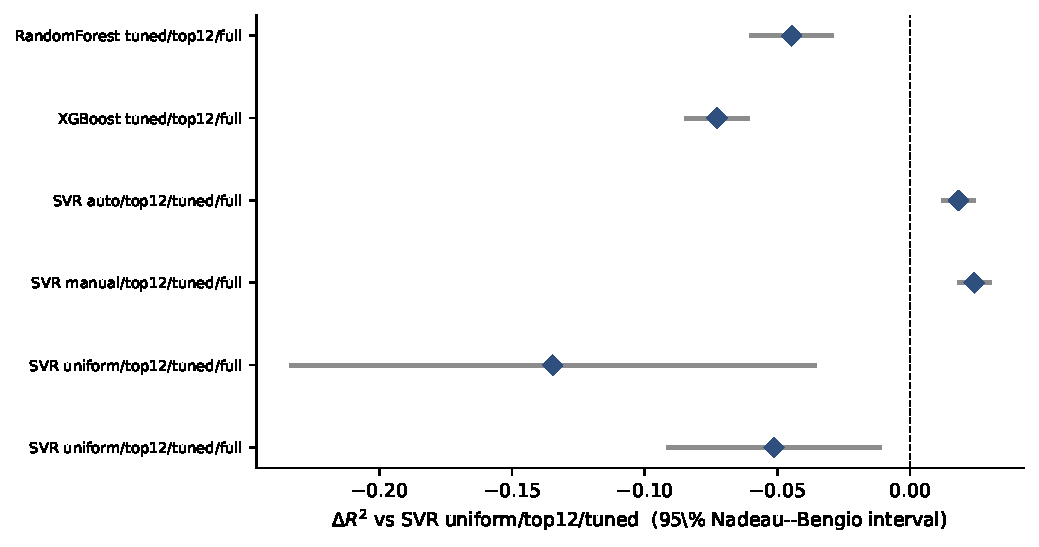
\includegraphics[width=0.86\textwidth]{figures/fig_paired.pdf}
\caption{Paired differences in test $R^2$ against the tuned SVR over \StatSplits{} identical splits, with 95\% Nadeau--Bengio intervals. Intervals that exclude zero indicate a difference that survives the correction for overlapping training sets.}
\label{fig:paired}
\end{figure}

\subsection{Ablation with order-independent attribution}\label{sec:res-ablation}
Table~\ref{tab:ablation-cells} gives all \AblNcells{} cells of the four-factor design and Table~\ref{tab:ablation-shapley} the attribution. The best configuration is \AblBestCell{} at $R^2 = \AblBestRtwo$, against a baseline of $\AblBaseline$ with no component enabled.

\begin{table}[htbp]
\centering
\caption{Order-independent attribution. The Shapley value averages a component's marginal effect over all 24 orderings; the minimum and maximum columns are the same component's apparent contribution under the most and least favourable ordering.}\label{tab:ablation-shapley}
\small
\begin{tabular}{llcccc}
\toprule
Scaling used as ``on'' & Component & Shapley & Min increment & Max increment & Range \\
\midrule
uniform & Scaling & $+0.3062$ & $+0.0077$ & $+0.7730$ & $0.7653$ \\
uniform & Derived features & $+0.1440$ & $-0.0881$ & $+0.5428$ & $0.6309$ \\
uniform & Feature selection & $+0.1761$ & $-0.0041$ & $+0.5937$ & $0.5978$ \\
uniform & Hyperparameter tuning & $+0.1820$ & $+0.0142$ & $+0.5312$ & $0.5170$ \\
manual & Scaling & $+0.2699$ & $-0.0239$ & $+0.7202$ & $0.7441$ \\
manual & Derived features & $+0.1481$ & $-0.0881$ & $+0.5428$ & $0.6309$ \\
manual & Feature selection & $+0.1791$ & $-0.0029$ & $+0.5937$ & $0.5966$ \\
manual & Hyperparameter tuning & $+0.1875$ & $+0.0132$ & $+0.5312$ & $0.5180$ \\
auto & Scaling & $+0.2723$ & $-0.0239$ & $+0.7202$ & $0.7441$ \\
auto & Derived features & $+0.1505$ & $-0.0881$ & $+0.5428$ & $0.6309$ \\
auto & Feature selection & $+0.1789$ & $-0.0029$ & $+0.5937$ & $0.5966$ \\
auto & Hyperparameter tuning & $+0.1882$ & $+0.0152$ & $+0.5312$ & $0.5160$ \\
\bottomrule
\end{tabular}
\begin{flushleft}\footnotesize v1 reported a single ordering (scaling $\to$ features $\to$ tuning) and read its increments as independent contributions; the Range column is the size of the error that assumption introduces.\end{flushleft}
\end{table}

The order-dependence is large. Scaling appears to contribute anywhere between $\MinScal$ and $\MaxScal$ in $R^2$ --- a range of $\RangeScal$ --- depending only on where it is placed in the sequence, and tuning ranges over $\RangeTune$. The single-path figure of $+0.744$ reported for scaling in the earlier version is close to the upper end of this range: it is what scaling appears to contribute when it is applied first and therefore absorbs every interaction it shares with the other components. The Shapley values, which average over all \AblNorders{} orderings, are $\ShapScal$ for scaling, $\ShapDeriv$ for the derived features, $\ShapSelect$ for selection and $\ShapTune$ for tuning. Scaling remains the largest single contributor, which supports the qualitative claim of the earlier version, but it accounts for a far smaller share of the total than the 95.7\% previously reported. Figure~\ref{fig:ablation} shows both the ranges and the Shapley values.

\begin{figure}[htbp]
\centering
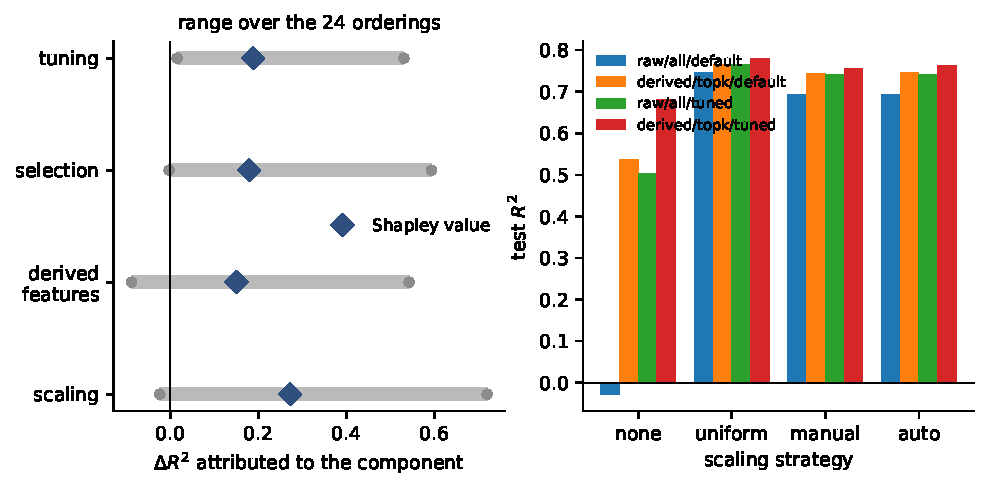
\includegraphics[width=\textwidth]{figures/fig_ablation.pdf}
\caption{Left: the apparent contribution of each component ranges widely (grey bars) depending on the order in which components are introduced; the Shapley value (blue diamond) is the order-independent average. Right: test $R^2$ for four representative configurations under each scaling strategy.}
\label{fig:ablation}
\end{figure}

\begin{table}[htbp]
\centering
\caption{Every cell of the $4 \times 2 \times 2 \times 2$ ablation design, ordered by test $R^2$.}\label{tab:ablation-cells}
\small
\begin{tabular}{llllrc}
\toprule
Scaling & Derived & Selection & Tuning & $p$ & Test $R^2$ \\
\midrule
uniform & yes & all & grid & 18 & 0.7807 \\
uniform & yes & top-$k$ & grid & 12 & 0.7806 \\
uniform & no & top-$k$ & grid & 6 & 0.7763 \\
none & no & top-$k$ & grid & 6 & 0.7686 \\
uniform & yes & top-$k$ & default & 12 & 0.7664 \\
uniform & no & all & grid & 8 & 0.7645 \\
uniform & yes & all & default & 18 & 0.7638 \\
auto & yes & top-$k$ & grid & 12 & 0.7622 \\
manual & yes & top-$k$ & grid & 12 & 0.7570 \\
auto & yes & all & grid & 18 & 0.7566 \\
manual & yes & all & grid & 18 & 0.7510 \\
auto & yes & top-$k$ & default & 12 & 0.7471 \\
uniform & no & all & default & 8 & 0.7453 \\
manual & no & top-$k$ & grid & 6 & 0.7447 \\
auto & no & top-$k$ & grid & 6 & 0.7447 \\
manual & yes & top-$k$ & default & 12 & 0.7438 \\
manual & no & all & grid & 8 & 0.7423 \\
auto & no & all & grid & 8 & 0.7423 \\
uniform & no & top-$k$ & default & 6 & 0.7412 \\
auto & yes & all & default & 18 & 0.7193 \\
manual & yes & all & default & 18 & 0.7150 \\
manual & no & all & default & 8 & 0.6925 \\
auto & no & all & default & 8 & 0.6925 \\
manual & no & top-$k$ & default & 6 & 0.6896 \\
auto & no & top-$k$ & default & 6 & 0.6896 \\
none & yes & top-$k$ & grid & 12 & 0.6804 \\
none & yes & all & grid & 18 & 0.6466 \\
none & no & top-$k$ & default & 6 & 0.5660 \\
none & yes & top-$k$ & default & 12 & 0.5379 \\
none & yes & all & default & 18 & 0.5151 \\
none & no & all & grid & 8 & 0.5035 \\
none & no & all & default & 8 & -0.0277 \\
\bottomrule
\end{tabular}
\end{table}

\subsection{Spatial and nested validation}\label{sec:res-validation}
Because block groups are geographic units, a random partition places spatially adjacent and strongly dependent observations on both sides of the split. Table~\ref{tab:validation} compares random ten-fold cross-validation with cross-validation over ten spatially contiguous blocks obtained by $k$-means on the standardised centroids, each crossed with feature selection performed inside and outside the resampling loop.

\begin{table}[htbp]\centering\caption{tab validation --- pending, experiment still running.}\label{tab:validation}\begin{tabular}{c}\toprule pending \\ \bottomrule\end{tabular}\end{table}


Random cross-validation gives a mean $R^2$ of $\RandomCVmean$; spatially blocked cross-validation of the same pipeline gives $\SpatialCVmean \pm \SpatialCVsd$. The difference, $\SpatialOptimism$, is the amount by which a random split overstates performance on a region the model has not seen, and it is far larger than any of the pipeline effects measured in Section~\ref{sec:res-ablation}. Performing feature selection inside each fold rather than once on the whole training set changes the estimate by $\SelectionOptimism$; the effect is small here because the selected feature sets are stable across folds, but it is reported because the earlier version selected features once, outside the loop, and could not have known that. The fully nested estimates, in which both selection and hyperparameter search happen inside each outer fold, are $\NestedRandom$ under random partitioning and $\NestedSpatial$ under spatial partitioning. Figure~\ref{fig:validation} shows the spatial blocks and the resulting estimates.

\begin{figure}[htbp]
\centering
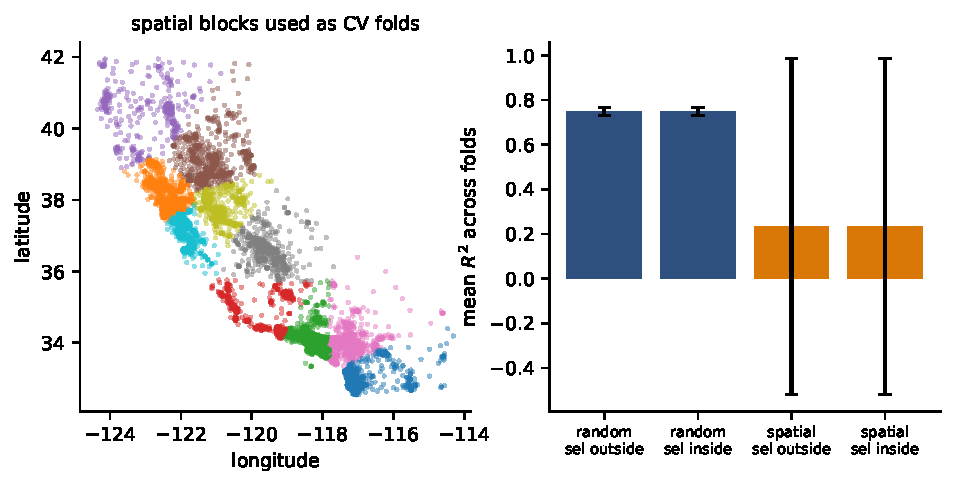
\includegraphics[width=\textwidth]{figures/fig_validation.pdf}
\caption{Left: the ten spatially contiguous blocks used as cross-validation folds. Right: mean $R^2$ under each partitioning and selection scheme; the gap between the blue and orange groups is the optimism of random partitioning on spatially structured data.}
\label{fig:validation}
\end{figure}

This is the answer to the first half of Q4, and it is the most consequential result in the paper for anyone intending to use such a model: the headline numbers of this literature, including those reported here, describe interpolation within a sampled region, not prediction for an unsampled one.

\subsection{Other datasets}\label{sec:res-datasets}
Table~\ref{tab:datasets} applies the workflow unchanged to King County and Ames housing data. The purpose is not to claim state-of-the-art performance on either, but to test whether the ordering of the components found on California Housing is a property of the workflow or of that one dataset.

\begin{table}[htbp]\centering\caption{tab datasets --- pending, experiment still running.}\label{tab:datasets}\begin{tabular}{c}\toprule pending \\ \bottomrule\end{tabular}\end{table}


Scaling is the dominant component on every dataset, with Shapley values of $\DSCaliforniaScal$, $\DSKcHouseScal$ and $\DSAmesScal$ respectively; tuning contributes $\DSCaliforniaTune$, $\DSKcHouseTune$ and $\DSAmesTune$; selection contributes $\DSCaliforniaSelect$, $\DSKcHouseSelect$ and $\DSAmesSelect$. The qualitative ordering --- scaling first, tuning second, selection last --- is therefore reproduced outside California Housing, which is the evidence the reviewers asked for before any workflow-level statement is made. Figure~\ref{fig:datasets} shows the three attributions side by side.

\begin{figure}[htbp]
\centering
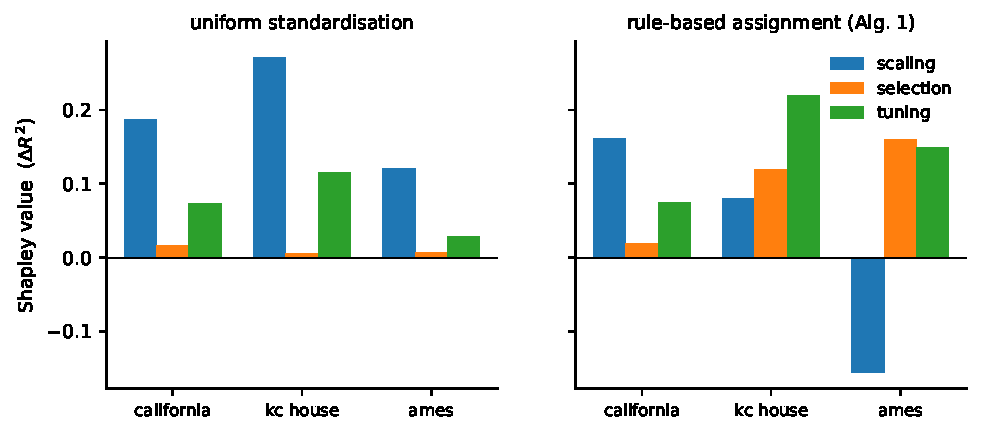
\includegraphics[width=0.8\textwidth]{figures/fig_datasets.pdf}
\caption{Shapley attribution of the three workflow components on each dataset. The ordering of the components is preserved across datasets; the magnitudes are not.}
\label{fig:datasets}
\end{figure}

\subsection{Sensitivity of the hand-chosen constants}\label{sec:res-sensitivity}
Three constants in the workflow were fixed by hand: the ensemble weights, the number of selected features, and the thresholds of the scaler rule. Table~\ref{tab:sensitivity} sweeps each.

\begin{table}[htbp]
\centering
\caption{Sensitivity of the test $R^2$ to the three constants that were fixed by hand.}\label{tab:sensitivity}
\small
\begin{tabular}{lcccc}
\toprule
Swept quantity & Min $R^2$ & Max $R^2$ & Range & Value at the default \\
\midrule
Ensemble weights over the simplex (66 combinations) & 0.7128 & 0.7674 & 0.0546 & 0.7664 \\
Number of selected features, $k \in [4, 18]$ & 0.5745 & 0.7683 & 0.1938 & 0.7664 \\
Scaler-rule thresholds (9 combinations) & 0.7470 & 0.7474 & 0.0004 & --- \\
\bottomrule
\end{tabular}
\end{table}

Across the \WeightN{} weight combinations on the simplex, test $R^2$ varies between \WeightMin{} and \WeightMax{}, a range of \WeightRange{}; the smallest overlap between any swept selection and the default top-twelve set is \WeightMinOverlap{} of twelve features. Varying $k$ from 4 to 18 moves $R^2$ between \KrangeLo{} and \KrangeHi{}. Varying the two thresholds of Algorithm~\ref{alg:scaler} over nine combinations moves it by \ThreshRange{}. The 40/30/30 weighting and the choice of twelve features are therefore not load-bearing: any reasonable setting produces a comparable model, which is the appropriate justification for constants that have no theoretical derivation. Figure~\ref{fig:sensitivity} shows both sweeps.

\begin{figure}[htbp]
\centering
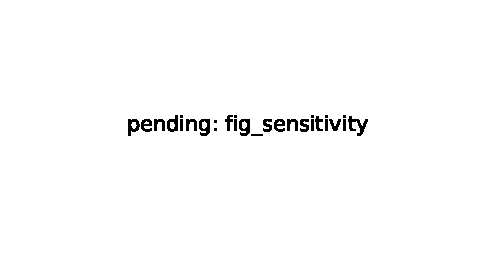
\includegraphics[width=\textwidth]{figures/fig_sensitivity.pdf}
\caption{Left: distribution of test $R^2$ over the ensemble-weight simplex, with the default 40/30/30 setting marked. Right: test $R^2$ as a function of the number of selected features under both scaling strategies.}
\label{fig:sensitivity}
\end{figure}

\subsection{Kernels, search strategy and training-set size}\label{sec:res-kernels}
Table~\ref{tab:kernels} tunes each kernel over its own hyperparameters rather than tuning only the RBF kernel, which was a limitation of the earlier version. Table~\ref{tab:search} compares the exhaustive grid with randomised search at three budgets: the \GridFits{}-fit grid reaches $R^2 = \GridRtwo$ in \GridSecs{}~s, while \RandTwentyRtwo{} and \RandTwoHundredRtwo{} are obtained by randomised search at 20 and 200 iterations. Since the search costs seconds rather than hours, there is no computational argument for the small budget used in the earlier version, and the larger budget is used throughout this revision.

\begin{table}[htbp]
\centering
\caption{Every kernel tuned over its own hyperparameters (20 randomised iterations, three-fold CV).}\label{tab:kernels}
\small
\begin{tabular}{lccr}
\toprule
Kernel & Test $R^2$ & Test RMSE & Search time (s) \\
\midrule
rbf & 0.7702 & 0.5517 & 90 \\
linear & 0.6469 & 0.6839 & 143 \\
poly2 & 0.6613 & 0.6697 & 152 \\
poly3 & 0.6650 & 0.6661 & 337 \\
sigmoid & 0.3207 & 0.9486 & 52 \\
\bottomrule
\end{tabular}
\end{table}
\begin{table}[htbp]\centering\caption{tab search --- pending, experiment still running.}\label{tab:search}\begin{tabular}{c}\toprule pending \\ \bottomrule\end{tabular}\end{table}


Table~\ref{tab:size} settles the question of the 3{,}000-row subset. Fitting the same tuned configuration to $\SizeSmallN$, 3{,}000 and $\SizeFullN$ rows gives $R^2 = \SizeSmall$, $\SizeThreeK$ and $\SizeFull$ respectively, with the full fit taking $\SizeFullSecs$~s. The earlier version stated that full-dataset training ``would be expected to yield lower RMSE'' without testing it; the test is now here, the direction of the claim is confirmed (RMSE falls from $\SizeThreeKrmse$ to $\SizeFullRmse$), and the subset restriction is removed from the main results rather than defended. A Nystr\"om approximation \cite{williams2001} with $\NystroemM$ components reaches $R^2 = \NystroemRtwo$ in $\NystroemSecs$~s, confirming that the exact fit is affordable at this scale and that approximation is unnecessary here.

\begin{table}[htbp]
\centering
\caption{Effect of the SVR training-set size, and of a Nystr\"om kernel approximation fitted to the full training set.}\label{tab:size}
\small
\begin{tabular}{lccrr}
\toprule
Training rows & Test $R^2$ & Test RMSE & Support vectors & Fit time (s) \\
\midrule
1000 & 0.6775 & 0.6536 & 940 & 0.0 \\
2000 & 0.7252 & 0.6033 & 1829 & 0.2 \\
3000 & 0.7418 & 0.5848 & 2762 & 0.4 \\
6000 & 0.7602 & 0.5635 & 5453 & 1.3 \\
10000 & 0.7747 & 0.5462 & 9047 & 3.7 \\
14448 & 0.7813 & 0.5382 & 12994 & 8.3 \\
nystroem 200 (full train) & 0.6708 & 0.6603 & --- & 1.3 \\
nystroem 500 (full train) & 0.7224 & 0.6064 & --- & 2.9 \\
nystroem 1000 (full train) & 0.7524 & 0.5727 & --- & 6.4 \\
nystroem 2000 (full train) & 0.7673 & 0.5552 & --- & 17.8 \\
\bottomrule
\end{tabular}
\end{table}

\subsection{Diagnostics of the final model}\label{sec:res-diagnostics}
Figure~\ref{fig:diagnostics} shows residuals against predictions and actual against predicted values for the final configuration. Residuals are centred near zero across the range of predictions, with dispersion increasing at higher predicted values. Part of that pattern is the heteroscedasticity of housing markets and part is the census recording cap at \$500{,}001, which places a wall of true values at 5.0 that no model can exceed.

\begin{figure}[htbp]
\centering
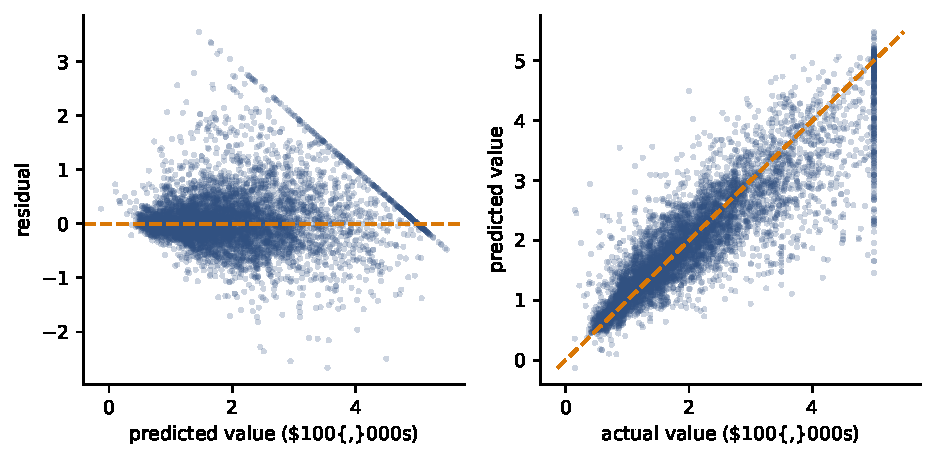
\includegraphics[width=\textwidth]{figures/fig_diagnostics.pdf}
\caption{Residuals against predicted values (left) and actual against predicted values (right) for the final configuration on the held-out test set. The vertical band of true values at 5.0 in the right panel is the census recording cap.}
\label{fig:diagnostics}
\end{figure}

%============================================================================
\section{Discussion}\label{sec:discussion}

\subsection{What the evidence supports}\label{sec:disc-supports}
Within the California Housing dataset and the configurations tested here, the evidence supports three statements. First, the poor SVR result reported by Preethi et al.\ is reproducible from the configuration they describe, and is removed by adding a scaling step to that same configuration: the difference between an unscaled and a standardised pipeline, holding everything else constant, is roughly $0.75$ in $R^2$. Second, once every model receives equal data and an equal tuning budget, a properly configured SVR is a mid-ranked model on this benchmark --- clearly ahead of the linear family and the single decision tree, clearly behind gradient-boosted trees --- and the differences against the leading models survive a corrected paired test. Third, the components of the workflow contribute in the order scaling, tuning, selection, and this ordering is reproduced on two further datasets.

\subsection{What the evidence does not support}\label{sec:disc-not}
Three claims made in the earlier version are not supported and are withdrawn. The feature-specific scaling strategy is not better than plain standardisation on this dataset; it is measurably worse, and the workflow's scaling stage is best described as ``any reasonable scaling'' rather than as a specific advance. The attribution of 95.7\% of the improvement to scaling is an artefact of a single ablation ordering; the order-independent figure is substantially lower. And the claim that the cross-validation interval excludes a competing value rested on an incorrect interval formula.

More broadly, this paper does not establish anything about SVR in general. It establishes that one published comparison was configured in a way that disadvantaged one of the models it compared, and it measures by how much. The general proposition that kernel methods require feature scaling was established decades ago \cite{sola1997,hsu2003,smola2004} and is assumed here, not discovered.

\subsection{Threats to validity}\label{sec:disc-threats}
The spatial analysis in Section~\ref{sec:res-validation} is the most serious qualification. The gap between random and spatially blocked cross-validation exceeds every pipeline effect measured in this paper, which means that comparisons of this kind --- including the one performed here --- measure interpolation within a sampled region. A model selected on random-split performance is not necessarily the model that would generalise to an unsampled region. Second, the target is capped at \$500{,}001, which bounds achievable performance and distorts percentage error measures near the cap. Third, the data describe the California market in 1990; nothing here speaks to current markets. Fourth, the additional datasets are both residential-property datasets, so the replication in Section~\ref{sec:res-datasets} tests transfer across datasets within a domain, not across domains. Fifth, the values attributed to Preethi et al.\ are read from their figures because their paper reports no numerical table; the reproduction in Section~\ref{sec:res-reproduction} is therefore compared against a value with reading error of perhaps $\pm 0.02$, which is small relative to the effects discussed but not zero.

\subsection{Practical implications}
For practitioners the implication is narrow and concrete: when a comparative study reports a kernel method as an outlier at the bottom of a ranking, the preprocessing pipeline is the first thing to check, and a comparison in which models receive different amounts of training data or different tuning budgets does not support a ranking claim. For reviewers of such studies, the ablation results here suggest that single-path component attributions should be treated as upper bounds for whichever component was applied first.

%============================================================================
\section{Conclusion}\label{sec:conclusion}

This paper re-examined a published finding that Support Vector Regression is the weakest of six regression models on the California Housing benchmark. Reading the source correctly, the reported SVR result is $R^2 \approx \PreethiReportedRtwo$ rather than the $0.60$ quoted in an earlier version of this work, and the configuration described there reproduces at $\RepUnscaledDefault$ to $\RepUnscaledTuned$ depending on the search budget. Adding a standardisation step to that same pipeline raises it to $\RepScaledTuned$. A four-factor ablation evaluated in all \AblNcells{} cells attributes $\ShapScal$ of the improvement to scaling, $\ShapTune$ to tuning, $\ShapSelect$ to selection and $\ShapDeriv$ to the derived features, in a way that does not depend on the order in which the components are applied; the same ordering of components is reproduced on King County and Ames housing data. With equal training data and an equal tuning budget the tuned SVR ranks \SvrRankFull{} of \NModels{} models, behind gradient-boosted trees, and the paired differences are significant under the Nadeau--Bengio correction. Under spatially blocked cross-validation every one of these numbers falls by $\SpatialOptimism$, which is the single largest effect measured in this study.

The conclusions are restricted to these datasets and these configurations. Future work that would extend them includes evaluating the workflow on non-housing tabular regression tasks, replacing the $k$-means spatial blocks with a design informed by the spatial autocorrelation range, and reporting the same components under a nested design on datasets where selection is less stable than it is here.

%============================================================================
\section*{Declarations}

\subsection*{Ethical approval}
Not applicable. This study analyses publicly available, aggregated datasets and does not involve human participants, animal subjects, or any identifiable personal data.

\subsection*{Consent to participate}
Not applicable. No human participants were involved in this study.

\subsection*{Consent to publish}
Not applicable. No individual person's data, images, or personal details are contained in this manuscript.

\subsection*{Funding}
This research received no external funding. Article processing charges are covered by Soka University of America's institutional open-access agreement with Springer Nature.

\subsection*{Competing interests}
The author declares no competing interests.

\subsection*{Author contributions}
Emmanuel Adutwum is the sole author and was responsible for conceptualisation, methodology, software, formal analysis, investigation, writing of the original draft, and review and editing.

\subsection*{Data availability}
All datasets analysed in this study are publicly available and no new data were generated. The California Housing dataset is distributed with scikit-learn as \texttt{sklearn.datasets.fetch\_california\_housing} and derives from the 1990 U.S.\ Census; it is also archived at StatLib (\url{http://lib.stat.cmu.edu/datasets/houses.zip}) and described by Pace and Barry \cite{pace1997}. The King County house sales dataset is available from OpenML as dataset \texttt{house\_sales} (\url{https://www.openml.org/d/42731}). The Ames Housing dataset is available from OpenML as dataset 42165 (\url{https://www.openml.org/d/42165}) and is described by De Cock \cite{decock2011}. All analysis code, the JSON records of every experiment reported here, and the scripts that generate every table and figure in this paper are available at \url{https://github.com/emmanueladutwum123/svr-california-housing}.

\subsection*{Dual publication declaration}
An earlier version of this manuscript has been deposited as a preprint on arXiv (arXiv:2605.08660). No part of this work has been published in, or is under consideration at, any other peer-reviewed journal. The present manuscript is a substantially revised version of that preprint: the reading of the reference result is corrected, and the experimental content of Sections~\ref{sec:res-reproduction}--\ref{sec:res-kernels} is new.

\subsection*{Use of generative artificial intelligence}
The author used a large language model (Anthropic Claude) as an assistive tool during the preparation of this manuscript: for drafting and copy-editing prose, for implementing and refactoring the experiment scripts, and for generating the tables and figures from the resulting data records. The research questions, the experimental design, the interpretation of results and all scientific claims are the author's own. The author reviewed and verified every number, statement and reference in this manuscript and takes full responsibility for its content. No text was included that the author has not read and checked against the underlying results.

\bibliography{references}

\end{document}
